\documentclass[11pt]{article}
% Shared preamble for the Carry-Adder Wall paper series.
% Each paper does:  % Shared preamble for the Carry-Adder Wall paper series.
% Each paper does:  % Shared preamble for the Carry-Adder Wall paper series.
% Each paper does:  \input{../../shared/preamble}
\usepackage[margin=1in]{geometry}
\usepackage{amsmath, amssymb, amsthm}
\usepackage{microtype}
\usepackage{graphicx}
\usepackage[hidelinks]{hyperref}

\newtheorem{theorem}{Theorem}
\newtheorem{corollary}{Corollary}
\newtheorem{lemma}{Lemma}
\theoremstyle{remark}
\newtheorem*{remark}{Remark}

\newcommand{\Mhash}{\mathsf{M}}
\newcommand{\SHA}{\mathrm{SHA\text{-}256}}
\newcommand{\SHAd}{\mathrm{SHA\text{-}256d}}
\newcommand{\MAJ}{\mathrm{MAJ}}
\newcommand{\Ch}{\mathrm{Ch}}
\newcommand{\Maj}{\mathrm{Maj}}
\newcommand{\bigO}{\mathcal{O}}

\usepackage[margin=1in]{geometry}
\usepackage{amsmath, amssymb, amsthm}
\usepackage{microtype}
\usepackage{graphicx}
\usepackage[hidelinks]{hyperref}

\newtheorem{theorem}{Theorem}
\newtheorem{corollary}{Corollary}
\newtheorem{lemma}{Lemma}
\theoremstyle{remark}
\newtheorem*{remark}{Remark}

\newcommand{\Mhash}{\mathsf{M}}
\newcommand{\SHA}{\mathrm{SHA\text{-}256}}
\newcommand{\SHAd}{\mathrm{SHA\text{-}256d}}
\newcommand{\MAJ}{\mathrm{MAJ}}
\newcommand{\Ch}{\mathrm{Ch}}
\newcommand{\Maj}{\mathrm{Maj}}
\newcommand{\bigO}{\mathcal{O}}

\usepackage[margin=1in]{geometry}
\usepackage{amsmath, amssymb, amsthm}
\usepackage{microtype}
\usepackage{graphicx}
\usepackage[hidelinks]{hyperref}

\newtheorem{theorem}{Theorem}
\newtheorem{corollary}{Corollary}
\newtheorem{lemma}{Lemma}
\theoremstyle{remark}
\newtheorem*{remark}{Remark}

\newcommand{\Mhash}{\mathsf{M}}
\newcommand{\SHA}{\mathrm{SHA\text{-}256}}
\newcommand{\SHAd}{\mathrm{SHA\text{-}256d}}
\newcommand{\MAJ}{\mathrm{MAJ}}
\newcommand{\Ch}{\mathrm{Ch}}
\newcommand{\Maj}{\mathrm{Maj}}
\newcommand{\bigO}{\mathcal{O}}


\title{\textbf{Carry Depth:\\
A Circuit-Independent Coordinate of ARX, and the One-Round Advantage Cliff}}
\author{Peter Hollows}
\date{\today}

\begin{document}
\maketitle

\begin{abstract}
The hardness of SHA-256d mining reduces, by the accounting of the first
paper in this series~\cite{paperI}, to a single question: whether the round
function admits a local shortcut that resolves the output without resolving
the carries on the path. We give that question a coordinate. The carry
chain of modular addition is the only operation in $\SHA$ whose
nonlinearity couples bit positions, so we define \emph{carry depth}, the
number of modular-addition layers on the dependency path between a
controllable input and a target output, and compute it exactly for $\SHAd$
by static dataflow analysis: $386$ layers. We then measure how far local
structure actually reaches. A hand-built carry-aware score predicts a
downstream output byte with selection advantage $0.886$ one adder layer
away, and that advantage falls below detection ($\le 0.0011$, consistent
with zero) one round deeper: a cliff, with no geometric tail. We account
for the cliff through the carry chain's spectral structure (Holte's matrix,
contraction rate $\tfrac12$ fixed by the base), separating the geometric
per-bit decay from the per-round mixing that produces the reset, and we
corroborate the cost reading with an exact-solver boundary, where Z3 nonce
recovery cliffs by more than three orders of magnitude at round $11$. The
$386$-layer separation is therefore wide: the strongest local attack we
tested expires about $100$ rounds before the output.
\end{abstract}

% =====================================================================
\section{Introduction}
% =====================================================================

The companion paper~\cite{paperI} bounds Bitcoin mining from two sides. The
per-candidate work is confined to three known sharing regions, and the
candidate count is locked at $2^{D}$ in the ideal model and reduced, in the
standard model, to a SHA-256 distinguisher. That accounting localizes the
entire residual to one object: a global algebraic shortcut that reads the
output without resolving the carries on the path. It does not say whether
such a shortcut exists. This paper studies that question structurally.

We make three contributions. First, we isolate the carry chain of modular
addition as the sole position-coupling nonlinearity of $\SHA$, so that the
difficulty of local prediction is exactly the difficulty of resolving
carries (Sections~\ref{sec:nonlin}--\ref{sec:coupling}). Second, we turn
this into \emph{carry depth}, an exact, implementation-invariant coordinate
counting carry layers along the input-to-output dataflow, and compute it at
$386$ for $\SHAd$ (Sections~\ref{sec:markov}--\ref{sec:accounting}). Third,
we measure the reach of local structure on real reduced $\SHA$ and find a
one-round cliff (Section~\ref{sec:anchor}), explain it through the carry
chain's spectral structure (Section~\ref{sec:scales}), and corroborate the
cost interpretation with an exact-solver boundary
(Section~\ref{sec:sat}). The separation between the $386$-layer depth and
the one-layer reach is what makes the residual of~\cite{paperI} a thin
target rather than a wide one.

% =====================================================================
\section{Carries are the entire nonlinearity of addition}\label{sec:nonlin}
% =====================================================================

For $c = a + b \bmod 2^{n}$, define the carry vector $\gamma$ by
$\gamma_0 = 0$ and $\gamma_{i+1} = \MAJ(a_i,b_i,\gamma_i)$. Then bit by
bit,
\[
  c_i = a_i \oplus b_i \oplus \gamma_i,
  \qquad\text{i.e.}\qquad
  a + b = a \oplus b \oplus \gamma(a,b).
\]
The $a\oplus b$ term is $\mathrm{GF}(2)$-linear, and \emph{all} nonlinear,
cross-position behaviour of addition is carried by $\gamma$. If $\gamma$
were known, addition would be pure \textsc{xor}, that is, linear. Fixing
every nonlinear-gate output (each carry bit, each $\Ch$ or $\Maj$ term)
collapses $\SHAd$ to a $\mathrm{GF}(2)$-affine map, and finding an input
that hits the target becomes a solvable linear system. Hardness is the cost
of resolving carries.

% =====================================================================
\section{Carries are the only position-coupling nonlinearity}\label{sec:coupling}
% =====================================================================

Classify each $\SHA$ operation by how it moves information:

\begin{center}
\begin{tabular}{lcc}
\hline
operation & linear over $\mathrm{GF}(2)$? & couples bit positions?\\
\hline
rotations, shifts, \textsc{xor}, $\Sigma_0,\Sigma_1,\sigma_0,\sigma_1$ & yes & linearly\\
$\Ch$, $\Maj$ & no (degree $2$) & no; bit-local ($\text{out}_i$ sees only $\text{in}_i$)\\
modular $+$ & no & \textbf{yes}; $\text{out}_i$ depends on all $\text{in}_{<i}$\\
\hline
\end{tabular}
\end{center}

The modular adder is the unique operation whose own nonlinearity couples
different bit positions: a high output bit depends on all lower input bits,
through the carry chain. ($\Ch$ and $\Maj$ are nonlinear but bit-local;
they inject no carry.) The round function is a bijection on the state
(SHACAL-2, invertible given the message word), so the adder destroys no
information. What it removes is \emph{locality}: the high bits of a sum
cannot be read without resolving the entire low-side carry chain.

% =====================================================================
\section{The carry Markov chain and Holte's matrix}\label{sec:markov}
% =====================================================================

Exploitable structure contracts with carry distance rather than merely
becoming unknown, and under an idealizing assumption the contraction has a
precise rate. For a single adder with operand bits $a_i,b_i$ \emph{uniform
and independent}, the carry is a two-state Markov chain $\gamma_{i+1} =
\MAJ(a_i,b_i,\gamma_i)$ with
\[
  \Pr[\gamma_{i+1}{=}1\mid \gamma_i{=}0] = \tfrac14,
  \qquad
  \Pr[\gamma_{i+1}{=}1\mid \gamma_i{=}1] = \tfrac34,
\]
that is, transition matrix $\left(\begin{smallmatrix}3/4 & 1/4\\ 1/4 &
3/4\end{smallmatrix}\right)$, stationary $(\tfrac12,\tfrac12)$, second
eigenvalue $\tfrac12$. Starting from the known $\gamma_0 = 0$, the bias
decays geometrically,
\[
  \Pr[\gamma_i = 0] = \tfrac12 + 2^{-(i+1)}.
\]
This is Holte's carry matrix~\cite{holte}. In base $2$, summing $k$
operands gives a $k$-state carry chain on $\{0,\dots,k-1\}$ whose
eigenvalues are exactly $\{2^{-j}:0\le j<k\}$ (the same matrix governs the
base-$2$ riffle shuffle~\cite{diaconisfulman}), so the second eigenvalue,
and hence the per-bit contraction rate, is $\tfrac12$ \emph{independent of
the operand count}. Extra operands introduce only faster-decaying modes;
the gap is fixed by the base, never by $k$. The carry-in becomes a fair
coin about $i$ positions above the anchor, and chaining adders composes
these contractions, which suggests that exploitable advantage decays as
roughly $2^{-\Theta(\text{carry depth})}$, where carry depth counts the
modular-add layers between the bits an attacker controls and the target
bit. The uniform-independent assumption does not hold inside $\SHA$, where
state words are structured and correlated, so this is a heuristic and a
prediction to test rather than a theorem; Section~\ref{sec:anchor} measures
the actual decay. This carry recurrence is precisely the finite state of
the addition viewed as an S-function~\cite{sfunction}, the modern framework
for ARX differential analysis~\cite{arx}, in which difference propagation
through modular addition is governed entirely by the carry state machine.

% =====================================================================
\section{Depth accounting: SHA-256d is 386 layers}\label{sec:accounting}
% =====================================================================

Carry depth is the structural coordinate of the proof-of-work function
space: a two-round reduced hash is solvable because its input-to-target
depth is $\bigO(1)$, whereas full $\SHAd$ sits hundreds of layers past
that. We compute the coordinate exactly by static dataflow analysis (no
hash evaluation; see \texttt{repro/carry\_depth.py}). We treat the block-1
message words as the source inputs (the miner controls them through the
nonce, the extranonce-driven Merkle root, the version, and the timestamp),
use the minimum-depth associative tree for each multi-operand sum
(conservative, since it credits the attacker with the shallowest legal
circuit), and count $\Ch$ and $\Maj$ as depth $0$ (they inject no carry, so
the figure is a \emph{floor} on the nonlinear separation, ignoring their
additional bit-local nonlinearity). The figure is convention-dependent: a
sequential or nonce-only accounting gives a somewhat larger number, so the
minimum-depth value below is the conservative choice.

\begin{center}
\begin{tabular}{lr}
\hline
quantity & value\\
\hline
one compression ($64$ rounds $+$ feed-forward) & $194$ adder layers\\
$\SHAd$ input$\to$output adder depth (min-tree) & $\mathbf{386}$\\
per-round increment & $\approx 3$ layers\\
modular adds on the path & $1200$\\
carry bits ($\approx 31$ per $32$-bit add) & $\approx 37{,}200$\\
\hline
\end{tabular}
\end{center}

The two feed-forwards and the second hash each act as an independent carry
reset (a fresh full-width operand), which is why they contribute more
separation than their round count alone would suggest;
Figure~\ref{fig:depth} traces the profile.

\begin{figure}[t]
\centering
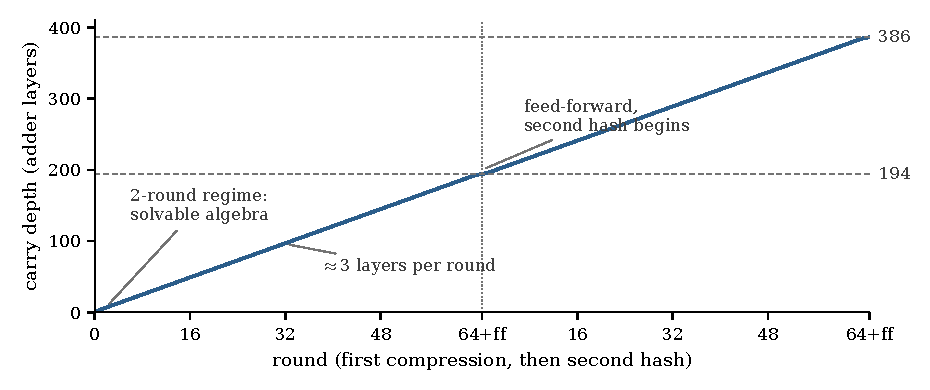
\includegraphics{figures/fig_depth_profile.pdf}
\caption{Carry depth along the SHA-256d dataflow, from the minimum-depth
accounting of \texttt{repro/carry\_depth.py}. The 64 rounds of the first
compression lift the state by about three adder layers each; the
feed-forwards and the second hash add full-width carry resets, reaching
$386$ layers from controllable input to output.}
\label{fig:depth}
\end{figure}

% =====================================================================
\section{The anchor sweep: a one-round cliff}\label{sec:anchor}
% =====================================================================

The depth fixes the exponent's base count ($386$); the margin is
$386\cdot\log_2(1/\rho)$, where $\rho$ is the advantage retained per adder
layer. We measure $\rho$ directly on real reduced $\SHA$ (see
\texttt{repro/anchor\_sweep.py}). The carry-aware score
$(T_1\!\gg\!24)+(T_2\!\gg\!24)$, read at an interior round, strongly
predicts that the top byte of $\mathtt{state}[0]$ is small one layer
downstream, and we measure how that control decays as the observed target
moves deeper. Over $24$ message stems (header-prefix stand-ins; see the
code for the simplified setup) and $2^{22}$ candidates each (standard error
on the mean advantage $\approx 10^{-3}$):

\begin{center}
\begin{tabular}{lc}
\hline
depth from read point & retained advantage\\
\hline
$1$ adder layer (same round) & $0.8856 \pm 0.0005$\\
one round deeper ($\approx 3$ layers) & $\le 0.0011$ (consistent with $0$)\\
\hline
\end{tabular}
\end{center}

The advantage \emph{cliffs} (Figure~\ref{fig:cliff}): it falls from $0.886$
to undetectable within a single round. There is no geometric tail to fit;
$\rho \approx 0$, a one-layer reset. The mechanism is explicit: at the next
round $\mathtt{state}[0]$ enters $\Sigma_0$, whose rotations scatter the
controlled top byte across all bit positions, and it is then re-randomized
by a fresh carry chain, so the controlled structure is delocalized off the
top-byte observable in one round. The information is preserved (the round
is invertible); the accessibility is destroyed.

\begin{figure}[t]
\centering
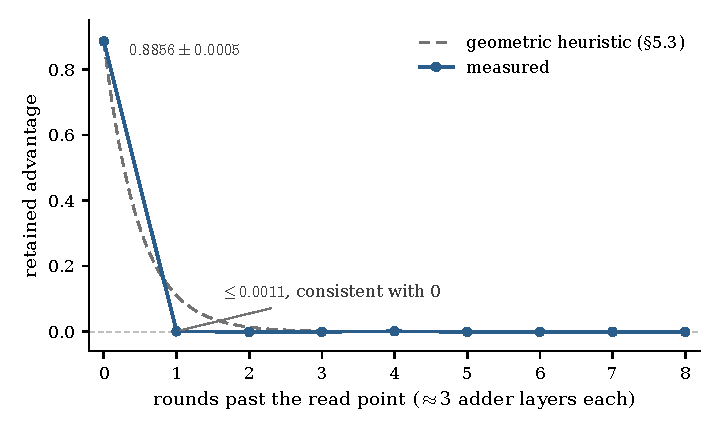
\includegraphics{figures/fig_anchor_cliff.pdf}
\caption{The anchor sweep: selection advantage of the carry-aware score
read $j$ rounds past the read point, against the geometric decay suggested
by the carry Markov heuristic of Section~\ref{sec:markov}. The measurement
returns a cliff rather than a slope; past one round every value sits within
the $\approx 10^{-3}$ detection limit of zero.}
\label{fig:cliff}
\end{figure}

\paragraph{The combined statement.}
The target output sits $386$ adder layers from the controllable header
inputs, while the strongest local advantage we measured has reach of about
one layer and is dead within a single round ($\approx 3$ layers). The
margin therefore does not rest on a thin $\rho^{386}$ extrapolation; the
advantage is already gone roughly $100$ rounds before the output. We
deliberately do not compound the measured one-sided bound
$\rho_{\text{round}}\le 0.0011$ (a $2\sigma$ upper bound on the
deeper-round mean advantage) across the remaining rounds: that bound is a
detection limit consistent with $\rho=0$, not a measured decay rate, and
multiplying it would manufacture a precise-looking exponent from a null
result. The honest statement needs no extrapolation, since the advantage is
already below detection after a single round and $\SHAd$ applies $128$.

% =====================================================================
\section{Two decay scales}\label{sec:scales}
% =====================================================================

The Markov heuristic of Section~\ref{sec:markov} predicts a geometric
slope, $2^{-\Theta(\text{depth})}$, while the anchor sweep returns a cliff.
These are consistent once two different axes are separated.

The geometric $2^{-d}$ decay lives on the \emph{bit-position} axis within a
single addition: it is the carry chain mixing along its own length, the
contraction whose rate is the second eigenvalue $\tfrac12$. This is the
quantity that linear and differential cryptanalysis of one ARX step sees,
and it is a genuine slope.

The \emph{round} axis is different. One $\SHA$ round is not one step of that
chain. The controlled word enters $\Sigma_0$, three rotations combined by
\textsc{xor}, which scatters its top byte across all bit positions, and it
is then fed as one addend into a fresh full-width carry chain with
independent operands. That is a full mixing step, not a single contraction,
so the retained advantage from a fixed read point collapses to the noise
floor in one round rather than decaying as a per-round $\rho$. The naive
reading conflates one carry step with one round; the cliff is what a full
per-round mixing time looks like, and the $386$-layer depth is the count of
such steps to the output.

% =====================================================================
\section{The SAT-solver boundary at eleven rounds}\label{sec:sat}
% =====================================================================

Carry depth predicts a solving cost as well as a statistical reach. If
reading the target requires resolving about three carry layers per round, a
complete solver should see its work grow geometrically with the round
count. We measure this with an exact SMT solver, Z3~\cite{z3}. The
instance fixes the nonce as the single $32$-bit unknown $W_3$, takes the
state after $r$ rounds of the correct round function for a hidden true
nonce, and asks for a nonce reaching it; it is satisfiable by construction,
and the returned witness is verified against \texttt{hashlib}.

Across rounds the wall-clock cost (two independent seeds, external hard
deadlines) is $0.08\,\mathrm{s}$ at $8$ rounds, $6.3\,\mathrm{s}$ at $10$,
and a timeout beyond $7200\,\mathrm{s}$ at $11$, $12$, and $13$, with
$14$ rounds and above undecided at the budget. The cost grows about
$80\times$ per two rounds through round $10$, then jumps more than three
orders of magnitude between round $10$ and round $11$: a one-round cliff at
the eighth nonce-dependent round. Folklore held that the solver ``stops
returning somewhere between $12$ and $64$ rounds''; the single archived
$12$-round solve used a round function with a $\Sigma_1$ miscomputation
that weakens it, and on the correct circuit $12$ rounds does not return in
$6.4$ hours at about $50$ threads. The geometric growth and the cliff are
the cost-side image of the same carry composition the anchor sweep sees
statistically: about three adder layers per round, a conflict space that
grows like $2^{\Theta(\text{depth})}$.

% =====================================================================
\section{Relation to circuit-complexity measures}\label{sec:circuit}
% =====================================================================

Carry depth should not be conflated with the circuit measures it
superficially resembles. The closest prior notion is the carry-truncation
depth of Field and Jones~\cite{fieldjones}, who independently identify the
carry as the sole nonlinearity of ARX; their depth is a local approximation
parameter on a single addition, whereas carry depth is an exact, global
count of carry layers along the input-to-output dataflow of the whole
function. It is likewise distinct from the FHE/MPC notion of
\emph{multiplicative} (AND) \emph{depth}. The standard Bristol-Fashion
circuit for one $\SHA$ compression has AND-depth
$1607$~\cite{bristol,multdepth}, far above our $386$, because AND-depth
counts every nonlinear gate on the path, including the bit-local $\Ch$ and
$\Maj$ gates and every gate of a ripple-carry adder, while carry depth
counts only carry layers and assigns $\Ch$ and $\Maj$ depth $0$.
AND-depth is a property of a chosen circuit: the same modular
addition has linear AND-depth as ripple-carry but logarithmic depth as a
parallel-prefix adder~\cite{cla}, since the carry-merge operator is
associative, and published heuristics shrink a $128$-bit adder from
AND-depth $255$ to $9$ without altering its logic~\cite{multdepth}. Carry
depth counts the logical carry-dependency layers and is invariant to the
realization; it is a coordinate of the function, not of an implementation.
Nor is it multiplicative \emph{complexity}, a gate \emph{count} (an
$n$-bit adder needs exactly $n{-}1$ AND gates~\cite{boyarperalta}) carrying
no notion of depth.

% =====================================================================
\section{Reproduction and conclusion}\label{sec:repro}
% =====================================================================

Two quantitative results are reproducible from self-contained code, built
on a vendored minimal $\SHA$ verified bit-exact against \texttt{hashlib}.
\texttt{carry\_depth.py} computes the $386$-layer accounting by static
dataflow analysis (pure Python, no dependencies, instant).
\texttt{anchor\_sweep.py} measures the cliff ($0.886$ at depth one,
consistent with $0$ one round deeper); the full run uses
\texttt{numpy}/\texttt{cupy}, and a \texttt{-{}-pure}
standard-library path reproduces the cliff and a \texttt{hashlib} parity
check on any interpreter. The SAT boundary is reproducible from the Z3
nonce-recovery sweep.

The carry as the sole nonlinearity of ARX is known~\cite{fieldjones,arx,
sfunction}. The contribution here is to turn it into carry depth, an
explicit, circuit-independent coordinate of the proof-of-work function
space, to compute it exactly at $386$ for $\SHAd$, and to measure that the
strongest local advantage has reach of about one layer. The structural
separation is large, the measured reach is one layer, and the residual
isolated by the companion paper~\cite{paperI} is therefore a thin target:
any attack that beats brute force must reach across $386$ carry layers that
the natural local methods cross by one.

% =====================================================================
\begin{thebibliography}{99}

\bibitem{paperI}
P.~Hollows.
\emph{The Amortization Envelope: Where a SHA-256d Mining Advantage Can and
Cannot Live.}
Carry-Adder Wall series~I, 2026.

\bibitem{holte}
J.~M.~Holte.
\emph{Carries, Combinatorics, and an Amazing Matrix.}
American Mathematical Monthly 104(2), 1997.

\bibitem{diaconisfulman}
P.~Diaconis, J.~Fulman.
\emph{Carries, Shuffling, and an Amazing Matrix.}
American Mathematical Monthly 116(9), 2009.

\bibitem{sfunction}
N.~Mouha, V.~Velichkov, C.~De Canni\`ere, B.~Preneel.
\emph{The Differential Analysis of S-functions.}
SAC 2010.

\bibitem{arx}
H.~Lipmaa, S.~Moriai.
\emph{Efficient Algorithms for Computing Differential Properties of
Addition.}
FSE 2001.

\bibitem{fieldjones}
R.~E.~Field, B.~C.~Jones.
\emph{Using Carry-Truncated Addition to Analyze Add-Rotate-Xor Hash
Algorithms.}
2013, \texttt{arXiv:1303.4448}.

\bibitem{bristol}
N.~P.~Smart et al.
\emph{`Bristol Fashion' MPC Circuits.}
\texttt{https://nigelsmart.github.io/MPC-Circuits/}.

\bibitem{multdepth}
P.~Aubry, S.~Carpov, R.~Sirdey.
\emph{Faster Homomorphic Encryption is not Enough: Improved Heuristic for
Multiplicative Depth Minimization of Boolean Circuits.}
CT-RSA 2020.

\bibitem{cla}
T.~G.~Draper, S.~A.~Kutin, E.~M.~Rains, K.~M.~Svore.
\emph{A Logarithmic-Depth Quantum Carry-Lookahead Adder.}
Quantum Inf.\ Comput.\ 6(4), 2006.

\bibitem{boyarperalta}
J.~Boyar, R.~Peralta.
\emph{Tight Bounds for the Multiplicative Complexity of Symmetric
Functions.}
Theoretical Computer Science 396, 2008.

\bibitem{z3}
L.~de Moura, N.~Bj\o rner.
\emph{Z3: An Efficient SMT Solver.}
TACAS 2008.

\end{thebibliography}

\end{document}
